\chapter{Modelowanie procesu}
	\label{ch:mod}
	
	\section{Opóźnienie}
		\label{sec:tau}
		
		W celu zdefiniowania opóźnienia $\tau$ procesu zasymulowaliśmy go dla pojedynczego skoku sterowania. Wyniki symulacji przedstawione są na wykresie \ref{fig:tau}. Skok sterowania nastąpił w 5 kroku działania programu, natomiast wyjście procesu zmieniło się dopiero w kroku 8. Oznacza to, że poszukiwane przez nas opóźnienie wynosi $\tau = 3$. Użyty przez nas skrypt to $tauwiz.m$.
		
		\begin{figure}[h!]
			\centering
			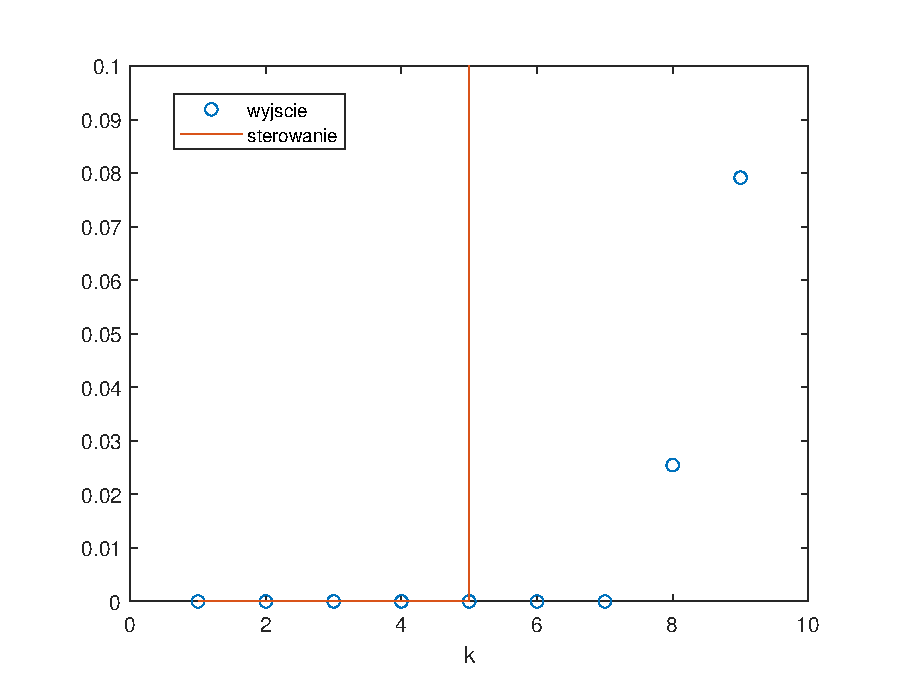
\includegraphics[width=\linewidth]{img/tau_wizualizacja.eps}
			\caption{Wizualizacja opóźnienia procesu}
			\label{fig:tau}
		\end{figure}
	
	\newpage
	\section{Dobór liczby neuronów}
		\label{sec:neurony}
		
		W celu dobrania odpowiedniej liczby neuronów dla sieci zastosowaliśmy wielokrotne uczenie z użyciem programu $sieci.exe$. Dla każdej ilości neuronów ukrytych od 1 do 10 dokonaliśmy 5 procesów uczenia za pomocą algorytmu BFGS z wykorzystaniem rekurencji. W tym celu wykorzystaliśmy skrypt $modelowanie.m$. Najmniejszy uzyskany błąd uczenia wraz ze skojarzonym z nim błędem weryfikacji przedstawiony został w tabeli poniżej. Najmniejszy błąd dla obydwu zbiorów występuje dla 9 neuronów. Ostatecznie jednak zdecydowaliśmy się na użycie sieci z pięcioma neuronami ukrytymi. Powodem tego jest mała poprawa w stosunku do większych ilości neuronów oraz chęć zmniejszenia nakładu obliczeń. Dodatkowo sieci o zbyt dużej ilości neuronów ukrytych mają tendencję do przetrenowywania się, w wyniku którego sieć przystosowuje się nie tyle do procesu co do samych danych uczących.
		
		\begin{table}[h!]
			\centering
			\begin{tabular}{c|l|l}
				Liczba neuronów&Błąd uczenia&Błąd weryfikacji\\\hline
				1&3.070626e+01&5.548815e+01\\\hline
				2&4.977413e-01&1.060318e+00\\\hline
				3&3.206039e-01&5.111444e-01\\\hline
				4&1.479096e-01&2.625729e-01\\\hline
				5&8.734595e-02&1.534512e-01\\\hline
				6&7.765994e-02&2.087909e-01\\\hline
				7&2.614618e-02&1.727668e-01\\\hline
				8&1.509561e-02&1.095385e-01\\\hline
				9&1.355132e-02&6.725641e-02\\\hline
				10&2.105601e-02&1.136051e-01\\\hline
			\end{tabular}
		\caption{Błędy modelu dla różnej ilości neuronów}
		\label{tab:neurony}
		\end{table}
		
	\section{Model z algorytmu BFGS}
		\label{sec:bfgs}
		
	\section{Symulacja modelu z algorytmu BFGS}
		\label{sec:bfgs_sym}
		
	\section{Model z algorytmu najszybszego spadku}
		\label{sec:naj_sp}
		
	\section{Model z algorytmu BFGS z uczeniem bez rekurencji}
		\label{sec:bfgs_arx}
		
	\section{Symulacja modelu z algorytmu BFGS z uczeniem bez rekurencji}
		\label{sec:bfgs_arx_sym}
		
	\section{Model metodą najmniejszych kwadratów}
		\label{sec:mnk}